% \section{Introduction}

The light curves of spotted, rotating stars are often non-sinusoidal and
Quasi-Periodic (QP).
These stars vary in brightness due to active regions on their surfaces which
rotate in and out of view.
The non-sinusoidal quality is caused by the complicated surface spot patterns
and the quasi-periodicity is caused both by the finite lifetimes of these
active regions and the presence of differential rotation.
A strictly periodic sinusoid is therefore not a good representative
model for the light curves of FGK stars.
In an ideal world, a physical model of the stellar surface would be
conditioned on the data.
A physically realistic generative model would perfectly capture the
complexity of shapes within stellar light curves as well as the
quasi-periodic nature, allowing for extremely precise probabilistic period
recovery.
However, such physical models must have many free parameters in order to
accurately represent a stellar surface and these parameters are extremely
degenerate.
For example, as well as global stellar parameters such as inclination and
rotation period, each spot or active region should have (at minimum) a
longitude, latitude, size, temperature and lifetime.
Considering that many stars have on the order of hundreds of spots CITATION,
the number of free parameters quickly becomes unwieldy, especially if the
posterior PDFs of these parameters are explored with MCMC.
Simplified spot models, such as the one described in \citet{lanza}, where
only two spots are modelled, have produced successful results, however these
simplified models sacrifice some precision due to lack of model flexibility.
Instead of using a physical model for stellar light curves, we choose to use
an {\it effective} model.
One which captures the behaviour but is not physically motivated (although
the parameters of this model may be interpreted as physical ones).
An ideal effective model for the light curve of a spotted, rotating star is
one with a small number of non-degenerate parameters that is flexible enough
to perfectly capture non-sinusoidal, QP behaviour.
These requirements are perfectly fulfilled by a Gaussian process (GP) model.

GPs are commonly used in the machine learning community and increasingly used
in other scientific fields, for example biology and geophysics (where GP
regression is called `krigging').
They are useful in regression problems involving a stochastic process,
specifically when the probability distribution for the process is a
multi-variate Gaussian.
If the probability of obtaining a data set, generated by some process, is a
Gaussian in $N$ dimensions, where $N$ is the number of data points, that data
set can be described as and {\it with} a Gaussian process.

Gaussian process models parameterise the covariance between data points to
describe the data.
A kernel function provides the parameterisation of the covariance matrix.
For example, take the time-series in figure \ref{fig:GP_example}.
This is a \kepler\ light curve of Earth-like planet host Kepler-452, a G-type
star that rotates once every $\sim$ 15 days.
The variability visible in this time-series is typical of \kepler\ FGK stars.
It has been fit with a GP model, shown in orange.
Since GPs are flexible models, a range of kernel functions could be used to
describe the variability of Kepler-452.
For example, the simplest and most commonly used kernel function, the
'Squared Exponential' (SE) could produce an adequate fit to these data.
The SE kernel function is defined as,
\begin{equation}
k_{i,j} = A \exp \left(-\frac{(x_i - x_j)^2}{2l^2} \right).
\end{equation}
\label{eq:SE}
The SE kernel function has the advantage of being very simple---it has just
two parameters, $A$, the amplitude of covariance and $l$ the exponential
length scale of covariance decay.
If $l$ is large, two data points very far apart in $x$ will be tightly
correlated, and vice versa.
The SE kernel function may be an adequate model of the covariance in stellar
light curves, but it is not a `useful' one because it does not have a
parameter that controls a period.
In order to infer a rotation period, it is necessary to use a periodic kernel
function and to optimise the parameter that controls the period.
For this reason, I use the `Quasi-Periodic' (QP) kernel function for the
inference of stellar rotation periods.
The QP kernel function is written,
\begin{equation}
k_{i,j} = A \exp \left(-\frac{(x_i - x_j)^2}{2l^2} -
\frac{\sin(\frac{2\pi}{P})^2}{\Gamma^2} \right).
\end{equation}
\label{eq:QP}

\begin{figure}
\begin{center}
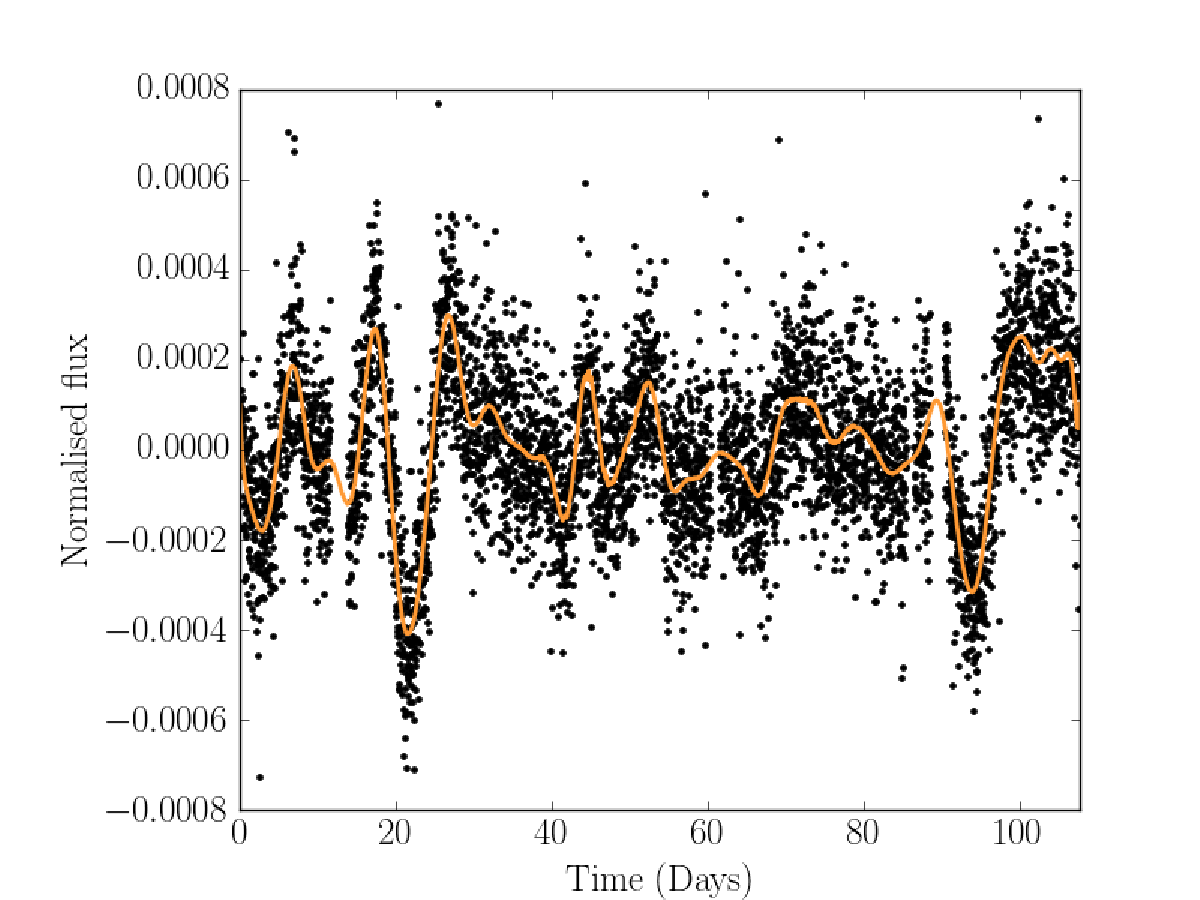
\includegraphics[width=6in, clip=true]{figures/Kepler452b.pdf}
\caption{Light curve of Kepler-452 b, a habitable-zone, Earth-sized planet
hosting G star \citep{jenkins}. The orange line shows a fit to the data using
a Gaussian process model with a QP covariance kernel function.}
\label{fig:GP_example}
\end{center}
\end{figure}

% Instead, we use an appropriate {\it effective} model: a Gaussian Process (GP)
% with a QP covariance kernel function.
% By modelling the covariance matrix of the light curve with a QP GP, we remain
% agnostic about model choice, whilst sampling directly from the posterior
% probability distribution function of the periodic parameter and marginalising
% over the other kernel hyperparameters.
% We simulated 300 light curves with a range of rotation periods and spot
% lifetimes and attempted to recover the rotation periods using three methods:
% our GP method, a sine-fitting periodogram method and an AutoCorrelation
% Function (ACF) method.
% The posterior probability distribution of the rotation period parameter was
% sampled using the affine invariant ensemble MCMC sampler, {\tt emcee} and the
% GP operations were performed using the {\tt george} python package This method
% produces rotation periods that are more precise than the periodogram and both
% more accurate and precise than the ACF method.

% \bibliographystyle{plainnat}
% \bibitem[Jenkins et al.(2015)]{jenkins}
% Jenkins, J.~M., Twicken, J.~D., Batalha, N.~M., et al.\ 2015, \aj, 150, 56
% \bibitem[Lanza et al.(2014)]{lanza}
% Lanza, A.~F., Das Chagas, M.~L., \& De Medeiros, J.~R.\ 2014, \aap, 564, A50

